%% CycleSafe:
%% Design Review Paper
%% ECE Capstone, Spring 2019

\documentclass[journal]{IEEEtran}

%% Packages for paper
\usepackage{cite}

% *** GRAPHICS RELATED PACKAGES ***
\usepackage[pdftex]{graphicx}
\graphicspath{{images/}}
\DeclareGraphicsExtensions{.pdf,.jpeg,.png}
\usepackage{tikz}
\usepackage[american voltages, arrowmos]{circuitikz}
\usetikzlibrary{math}

% *** MATH PACKAGES ***
\usepackage{amsmath}
\usepackage{physics}
\usepackage{siunitx}

% *** SPECIALIZED LIST PACKAGES ***
\usepackage{algorithmic}

% *** SUBFIGURE PACKAGES ***
\usepackage[caption=false,font=footnotesize]{subfig}

% *** FLOAT PACKAGES ***
\usepackage{float}
%\usepackage{fixltx2e}
% fixltx2e, the successor to the earlier fix2col.sty, was written by
% Frank Mittelbach and David Carlisle. This package corrects a few problems
% in the LaTeX2e kernel, the most notable of which is that in current
% LaTeX2e releases, the ordering of single and double column floats is not
% guaranteed to be preserved. Thus, an unpatched LaTeX2e can allow a
% single column figure to be placed prior to an earlier double column
% figure.
% Be aware that LaTeX2e kernels dated 2015 and later have fixltx2e.sty's
% corrections already built into the system in which case a warning will
% be issued if an attempt is made to load fixltx2e.sty as it is no longer
% needed.
% The latest version and documentation can be found at:
% http://www.ctan.org/pkg/fixltx2e


%\usepackage{stfloats}
% stfloats.sty was written by Sigitas Tolusis. This package gives LaTeX2e
% the ability to do double column floats at the bottom of the page as well
% as the top. (e.g., "\begin{figure*}[!b]" is not normally possible in
% LaTeX2e). It also provides a command:
%\fnbelowfloat
% to enable the placement of footnotes below bottom floats (the standard
% LaTeX2e kernel puts them above bottom floats). This is an invasive package
% which rewrites many portions of the LaTeX2e float routines. It may not work
% with other packages that modify the LaTeX2e float routines. The latest
% version and documentation can be obtained at:
% http://www.ctan.org/pkg/stfloats
% Do not use the stfloats baselinefloat ability as the IEEE does not allow
% \baselineskip to stretch. Authors submitting work to the IEEE should note
% that the IEEE rarely uses double column equations and that authors should try
% to avoid such use. Do not be tempted to use the cuted.sty or midfloat.sty
% packages (also by Sigitas Tolusis) as the IEEE does not format its papers in
% such ways.
% Do not attempt to use stfloats with fixltx2e as they are incompatible.
% Instead, use Morten Hogholm'a dblfloatfix which combines the features
% of both fixltx2e and stfloats:
%
% \usepackage{dblfloatfix}
% The latest version can be found at:
% http://www.ctan.org/pkg/dblfloatfix



%\ifCLASSOPTIONcaptionsoff
%  \usepackage[nomarkers]{endfloat}
% \let\MYoriglatexcaption\caption
% \renewcommand{\caption}[2][\relax]{\MYoriglatexcaption[#2]{#2}}
%\fi
% endfloat.sty was written by James Darrell McCauley, Jeff Goldberg and 
% Axel Sommerfeldt. This package may be useful when used in conjunction with 
% IEEEtran.cls'  captionsoff option. Some IEEE journals/societies require that
% submissions have lists of figures/tables at the end of the paper and that
% figures/tables without any captions are placed on a page by themselves at
% the end of the document. If needed, the draftcls IEEEtran class option or
% \CLASSINPUTbaselinestretch interface can be used to increase the line
% spacing as well. Be sure and use the nomarkers option of endfloat to
% prevent endfloat from "marking" where the figures would have been placed
% in the text. The two hack lines of code above are a slight modification of
% that suggested by in the endfloat docs (section 8.4.1) to ensure that
% the full captions always appear in the list of figures/tables - even if
% the user used the short optional argument of \caption[]{}.
% IEEE papers do not typically make use of \caption[]'s optional argument,
% so this should not be an issue. A similar trick can be used to disable
% captions of packages such as subfig.sty that lack options to turn off
% the subcaptions:
% For subfig.sty:
% \let\MYorigsubfloat\subfloat
% \renewcommand{\subfloat}[2][\relax]{\MYorigsubfloat[]{#2}}
% However, the above trick will not work if both optional arguments of
% the \subfloat command are used. Furthermore, there needs to be a
% description of each subfigure *somewhere* and endfloat does not add
% subfigure captions to its list of figures. Thus, the best approach is to
% avoid the use of subfigure captions (many IEEE journals avoid them anyway)
% and instead reference/explain all the subfigures within the main caption.
% The latest version of endfloat.sty and its documentation can obtained at:
% http://www.ctan.org/pkg/endfloat
%
% The IEEEtran \ifCLASSOPTIONcaptionsoff conditional can also be used
% later in the document, say, to conditionally put the References on a 
% page by themselves.


% *** PDF, URL AND HYPERLINK PACKAGES ***
\usepackage{url}
\usepackage{hyperref}
\hypersetup{
    urlcolor=blue
}

% *** OTHER PACKAGESS ***
\usepackage{booktabs} % for \toprule, \midrule, etc
\usepackage{tabularx}
\usepackage{pdfpages}

% correct bad hyphenation here
\hyphenation{op-tical net-works semi-conduc-tor}

%% Shortcuts
\newcommand{\slane}{s_\text{lane}}
\newcommand{\sbrake}{s_\text{brake}}
\newcommand{\lidar}{Garmin LIDAR-Lite v3}
\newcommand{\sonar}{HC-SR04}

%% Custom config
\DeclareSIUnit{\mph}{mph}
\DeclareSIUnit\lb{lb}
\sisetup{detect-all} % Use the environment font when calling siunitx

\begin{document}

% Do not put math or special symbols in the title.
\title{CycleSafe: A Technology-Assisted \\ Safety Jacket to Prevent Traffic Accidents}

\author{
    Benjamin~Huang,~\IEEEmembership{Electrical and Computer Engineering,~Carnegie Mellon University} \\
    Siddhanth~Lathar,~\IEEEmembership{Electrical and Computer Engineering,~Carnegie Mellon University} \\
    Michael~You,~\IEEEmembership{Electrical and Computer Engineering,~Carnegie Mellon University} \\
}

% The paper headers
\markboth{18-500 Design Review Report: 3/4/2019}%
{CycleSafe}

% make the title area
\maketitle

% As a general rule, do not put math, special symbols or citations
% in the abstract or keywords.
\begin{abstract}
Although biking is convenient way to travel, cyclists are at a high risk of accidents, where thousands of cyclists die every year. One reason is that cyclists have a limited number of safety options available, such as reflective vests and flashing lights, that give them little awareness of the road. CycleSafe is a comprehensive safety system on a bike, that alerts users through a wearable jacket when the cyclist is in a dangerous situation. The jacket notifies the user through a combination of visual, auditory and sensory feedback, and also features a large LED matrix that significantly increases the visibility of the rider compared to current cyclist safety products. CycleSafe aims to provide a safer biking experience by maximizing surrounding awareness to cyclists, while also increasing their visibility to other vehicles and their drivers.
\end{abstract}

\begin{IEEEkeywords}
Cyclist safety, wearable, real-time embedded system, LIDAR, haptic feedback
\end{IEEEkeywords}


\section{Introduction}
% The very first letter is a 2 line initial drop letter followed
% by the rest of the first word in caps.
% 
% form to use if the first word consists of a single letter:
% \IEEEPARstart{A}{demo} file is ....
% 
% form to use if you need the single drop letter followed by
% normal text (unknown if ever used by the IEEE):
% \IEEEPARstart{A}{}demo file is ....
\IEEEPARstart{E}{very} year, around 1,000 cyclists lose their lives and over 50,000 are injured in traffic accidents. Whereas cars are becoming safer, equipped with the latest safety features, biking technologies have remained mostly stagnant in the last few decades. This is a problem, especially because biking is becoming more popular in cities \cite{biking_popularity}, where 71\% of biking fatalities occur \cite{biking_crashes}. In particular, accidents are commonly caused by 5 factors - three of which are cyclists getting hit by 1) cars coming out of side streets, 2) cars turning into the side streets and 3) cars overtaking when a cyclists is moving left to avoid an obstacle \cite{biking_cases}. To prevent these accidents from happening, we present the CycleSafe, a system integrated with a wearable that helps keep bikers safe from these types of accidents by:

\begin{itemize}
    \item Helping you stay aware of your environment, giving danger warnings of lane drifting, blind spots and collision detection, and providing standard vehicle turn signals and brake lights, along with other communicative display signals.
    \item Navigation help, that reduces the need to look at your phone, and instead lets you focus your attention on the road.
    \item Gesture recognition, that reduces the need for large movements, and instead allows the user to make small movements to perform tasks, in order to reduce unsafe movement while biking.
\end{itemize}

The jacket also features many improvements to the cycling experience, such as glove warming, and on-demand music and call with your phone, features which current cyclist jackets on the market do not offer. To evaluate the effectiveness of the jacket under dangerous circumstances, we will conduct a simulation test in a closed test track. We are aiming to have $<$5\% false negatives, and $<$20\% false positives in 60 trial runs. We want to have a lower false negative than false positive because missing a dangerous condition is much worse than alerting the user where there are no dangers. More details about our testing can be found in \ref{specs:warning_thresholds}.

\section{Design Requirements}
\subsection{Mobile App}
The requirements for the mobile app are as follows:
\begin{itemize}
  \item Send data to the Raspberry Pi as inputs to the warning system logic. Data types include:
  \begin{itemize}
    \item Bicycle speed
    \item Current location
    \item Intersection data
  \end{itemize}
  \item Give the user live-time navigation instructions
  \item Give the user the ability to customize their notification settings
\end{itemize}
To test the data transfer, we will write a test program on the mobile app and the Raspberry Pi that works the following way:
\begin{enumerate}
    \item The mobile app sends a burst of pre-selected data
    \item The Raspberry Pi verifies the data is in the proper format and correct
\end{enumerate}
For navigation, we will test the app empirically, by choosing a series of locations to visit, and navigating to them on a bike with our mobile app giving live instructions.
For customization aspect of the app, we will write UI tests to make sure all buttons are working, settings are saved, and that they are actually sent to the jacket Arduino correctly. 
\subsection{The Jacket}
The requirements for the jacket are as follows:
\begin{itemize}
  \item Give the user warnings via peripherals, which include
  \begin{itemize}
    \item Piezo Buzzers (Auditory)
    \item Vibration Motors (Sensory)
    \item LEDs (Visual)
  \end{itemize}
  \item Give the user critical and less-critical warnings in time. These requirements can be found in Section \ref{specs:warning_thresholds}
  \item Make sure the LEDs are bright enough based on eCFR (Electronic Code of Federal Regulations) vehicle standards  \item Meet IPX4 waterproofing requirements
\end{itemize}

To test the peripherals on the jacket, we will write individual component unit testing code.
Specifically,
\begin{itemize}
    \item LED Strip: Send a series of patterns, and make sure that they appear correctly and bright enough.
    \item Piezo Buzzers: Send a series of beeps, and make sure they are loud enough and are happening at the correct times. 
    \item Vibration Motors: Send a series of vibration pulses, and make sure they are felt and are happening at the correct times
\end{itemize}
In order to verify the correct functionality of these tests, we will put the jacket on a user and have them respond yes or no to the above tests. For the LED strips, we have to match the eCFR standards\cite{light-brightness} which are
\begin{itemize}
    \item \SI{50}{\milli\candela} for tailights
    \item \SI{300}{\milli\candela} for turn signal
    \item \SI{300}{\milli\candela} for stoplights
\end{itemize}
We can test the brightness of the LEDs using a luminosity sensor.

In order to test the waterproofing, we will follow the IPX4 specification\cite{ipx-waterproofing}, and test according to the description:
\begin{equation}
    \textit{Protects from splashing water, no matter the direction}
\end{equation}
Once we have our jacket assembled, we will conduct a series of splash tests, and use the unit tests described earlier for individual components to evaluate the waterproofing effectiveness. 

\subsection{Warning Thresholds}
\label{specs:warning_thresholds}
The requirements for the CycleSafe system will be based on a maximum cycling speed of \SI{9}{\meter/\s} (about \SI{20}{\mph} or \SI{33}{\km/\hour}, which is high speed for a commuting cyclist averaging \SI{15}{\km/\hour} in some places \cite{cycling-speed}). Given this speed, we can determine the lead time necessary for a cyclist to react to dangers.

\subsubsection{Frontal warning}
With regard to frontal collisions, the necessary reaction time is fairly straightforward, since the cyclist simply needs sufficient time (or distance) to react and stop. From the maximum cycling speed, we can determine the cyclist's braking distance. In \cite{braking_distance}, the following formula is given to determine braking distance $\sbrake$, including perception and brake reaction time (the time needed to press the brakes):

\begin{align}
    \sbrake = \frac{v_b^2}{254(f \pm G)} + \frac{v_b}{1.4}
\end{align}

where $v_b$ is the velocity of the bicycle in \SI{}{\km/\hour}, $f$ is the coefficient of friction, and $G$ is the grade of the road (rise/run). The authors suggest using a coefficient of friction of 0.25 to account for wet weather. According to the author, the formula assumes a value of \SI{2.5}{\s} for perception and brake reaction time. However, the CycleSafe system is intended to reduce perception time, and hence \SI{2.5}{\s} would be an overestimate of total perception and brake reaction time. It would be useful to determine exactly how \SI{2.5}{\s} is distributed between perception and brake reaction time, since the system will not reduce brake reaction time but will reduce perception time significantly. In \cite{reaction-time}, a study is performed on human reaction and danger perception time for adult and child cyclists. The perception time for different scenarios in the study varies, but the scenario with the lowest average perception time has \SI{0.9}{\s}. As such, we can consider that we can likely discount about \SI{0.9}{\s} from the required total braking time.

At the assumed maximum cycling speed of \SI{9}{\meter/\s}, or \SI{32.4}{\km/\hour}, we have $\sbrake = \SI{27.3}{\meter}$ according to the formula. This is at least \SI{3}{\s} at the maximum speed. Discounting the perception time, we have a lead time of at least \SI{2.1}{\s} at maximum speed, or \SI{19}{\meter}, which we will set as the minimum required lead time for frontal collision warnings.

Additionally, the sensor should be able to resolve objects as small as open vehicle doors, a common cause of accidents \cite{biking_cases}. However, vehicle door size is not a good determining factor of the resolution since we want a lower bound, not an upper bound. We can consider that the cyclist will be travelling at least half a handlebar width away from parked vehicles, which would set the minimum size of a vehicle door obstruction at that length. Handlebar width is typically around \SI{40}{\cm}, so we can set a minimum resolution at \SI{20}{\cm}. There is still significant additional allowance in real scenarios since the cyclist will most likely not be cycling with the handlebar right up against parked vehicles, or anywhere close to it, especially if they are travelling at \SI{9}{\meter/\s}.

Testing of the frontal sensors, given the \SI{2.1}{\s} lead time and \SI{20}{\cm} resolution requirement, will follow the functional testing method described below. All tests will have cyclist speeds up to \SI{9}{\meter/\s} if possible (depending on the fitness of the cyclist). 

\begin{enumerate}
    \item \textit{Static obstacle test} (parked vehicle simulation). 10 trials in a closed course will be carried out, with varying cyclist speeds up to \SI{9}{\meter}. The obstacle will be a large square sheet of paper \SI{50}{\cm} in length, held at a height between \SI{50}{\cm} to \SI{100}{\cm} off the ground. The passing condition for these tests is that a warning is active starting between \SI{2.1}{\s} and \SI{3}{\s} before the cyclist contacts the sheet of paper. The cyclist will attempt to keep a constant speed, and if the cyclists' speed fluctuates more than \SI{1}{\meter/\s} within the alert duration the test will be voided.
    
    \item \textit{Sudden obstacle test} (vehicle door simulation). 10 trials in a closed course will be carried out. The obstacle will be a piece of cardboard \SI{20}{\cm} wide and \SI{50}{\cm} tall, held at a height between \SI{40}{\cm} to \SI{60}{\cm} off the ground, and rotated into the cyclist's path when the cyclist is not more than \SI{19}{\meter} away. The passing condition for these tests is that a warning is active within \SI{0.9}{\s} of the obstacle being placed in the way of the cyclist. The cyclist will attempt to keep a constant speed before the alert is active, and if the cyclists' speed fluctuates more than \SI{1}{\meter/\s} during that time the test will be voided. The cyclist may slow down or swerve once the alert is active.
    
    \item \textit{Moving obstacle test} (false positive test). 10 trials will be carried out with the cyclist pedalling on a trainer, to simulate the speed to the system. The obstacle will be a large square sheet of paper \SI{50}{\cm} in length, held at a height between \SI{50}{\cm} to \SI{100}{\cm} off the ground, moving towards the (now stationary) cyclist at speeds up to \SI{5}{\meter/\s}. Again, the passing condition for these tests is that a warning is active starting between \SI{2.1}{\s} and \SI{3}{\s} before the cyclist contacts the sheet of paper. The cyclist will attempt to keep a constant speed, and if the cyclists' speed fluctuates more than \SI{1}{\meter/\s} within the alert duration the test will be voided. In particular, this test determines if the system alerts the cyclist unnecessarily when the obstacle is not moving toward the cyclist, so the upper bound of \SI{3}{\s} is important.
\end{enumerate}

\subsubsection{Blind spot warning}
We determine the requirements for blind spot warnings assuming typical values. Firstly, lane width $\slane$ is approximately \SI{3}{\meter} \cite{lane_width}. We consider that larger lane width will make cycling safer since vehicles will not pass as close to the cyclist when overtaking. We also set a minimum cycling speed threshold at which the lane-change warning system provides guaranteed reaction time, which we set at \SI{5}{\meter/\s}. We also need to determine a maximum vehicle speed at which the warning provides guaranteed reaction time, which we set at \SI{20}{\meter/\s} (approx. \SI{45}{\mph}, the typical maximum speed limit on non-freeway urban roads). %TODO cite
The assumption of vehicles travelling at the speed limit is likely unrealistic, since vehicles often exceed the posted speed limit. However, in the absence of the speed limit it is difficult to place an upper bound on the maximum speed of a vehicle. While the calculations are based on the speed limit and thus CycleSafe system guarantees are given as such, the system will still function, albeit with reduced effectiveness, without such assumptions. It is inevitable that cyclists occasionally come into contact with reckless drivers, and in such scenarios we rely on a best-effort warning, instead of attempting to provide a quantitative guarantee.

To provide a blind spot warning to a cyclist changing lanes, the system must determine the time at which an oncoming vehicle will cross paths with a cyclist. Taking the minimum cycling speed of \SI{5}{\meter/\s} and vehicle speed of at most \SI{20}{\meter/\s}, an oncoming vehicle will approach at at most \SI{15}{\meter/\s}. In this case, we wish to provide the cyclist with \SI{2}{\s} reaction time to cancel or delay a lane change if necessary, more than enough for the cyclist to change direction (which is much quicker than braking). Note that we provided \SI{2.1}{s} for braking. This will set the requirement for the sensor's effective range at \SI{30}{\meter}.

Testing for the blind spot warning will be similar to the testing for the frontal collision warning. All tests will have cyclist speeds up to \SI{9}{\meter/\s} if possible (depending on the fitness of the cyclist), and the cyclist's left turn signal will be active throughout. The tests are outlined below.

\begin{enumerate}
    \item \textit{Standard lane change.} 10 trials will be carried out with the cyclist pedalling on a trainer, to simulate the speed to the system. A vehicle will come up behind the cyclist offset to the left by a distance between \SI{2}{\meter} and \SI{3}{\meter}, at speeds up to \SI{15}{\meter/\s} relative to the (stationary) cyclist. The passing condition for this test is that a notification is activated starting between \SI{2.5}{\s} and \SI{1.5}{\s} before the vehicle passes the cyclist, and a warning is activated between \SI{1.5}{\s} and \SI{0.5}{\s} before the vehicle passes the cyclist. Both these conditions must be true to pass the test. The cyclist will attempt to keep a constant speed, and if the cyclists' speed fluctuates more than \SI{1}{\meter/\s} after the notification the test will be voided.
    
    \item \textit{Standard lane change} (false positive). 10 trials will be carried out with the cyclist pedalling on a trainer, to simulate the speed to the system. A vehicle will come up behind the cyclist offset to the left by a distance between \SI{1.5}{\meter} and \SI{2.5}{\meter}, at speeds up to \SI{15}{\meter/\s} relative to the (stationary) cyclist but will slow down, going no quicker than \SI{7.5}{\meter/\s} when \SI{15}{\meter} away from the back of the cyclist, and will not overtake the cyclist or come any closer than \SI{5}{\meter} away from the back of the cyclist. The passing condition for this test is that a notification is activated but a warning is not activated. Both these conditions must be true to pass the test. The cyclist will attempt to keep a constant speed, and if the cyclists' speed fluctuates more than \SI{1}{\meter/\s} after the notification the test will be voided.
\end{enumerate}

\subsubsection{Right-turn cut-off warning}
For right-turn cut-off warnings when a vehicle is about to make a right turn into a side street in front of a cyclist, there is a large range of possible positions the vehicle may take in relation to the cyclist. However, the vehicle will always have to come into fairly close proximity to the cyclist, which we assume to be less than one lane width ($\slane$ = \SI{3}{\meter}). Therefore, the system should be able to detect vehicles within \SI{3}{\meter} of the cyclist in a \SI{180}{\degree} semi-circle on the left of the cyclist. This will also set the minimum distance at which proximity warnings to cars will activate.

This will be tested using the same method as the first standard lane change test, except that the turn signal will be off. The passing condition for this test is that the proximity signals are active when the vehicle is passing such that the shortest distance to the cyclist is less than \SI{3}{\meter}. There is no upper bound distance or time for this test since active proximity sensors do not harm the cyclist's trust in the system. 10 trials will be carried out for this test.

The testing for when vehicles cut into the cyclist's path ahead of the cyclist to turn right is subsumed under the car door simulation test. In case a car is about to directly impact the cyclist when turning right, no warning is given to the cyclist because there is no safer action the cyclist can take. Slowing down is not a safe action since it may cause problems for a driver who thinks the cyclist will be fast enough to clear a side street before the driver turns. Instead, the system protects against such occurrences using the proximity sensors and increasing the cyclist's awareness of the presence of a side street.

%TODO\subsection{Durability and Robustness}

\begin{figure*}
    \centering
    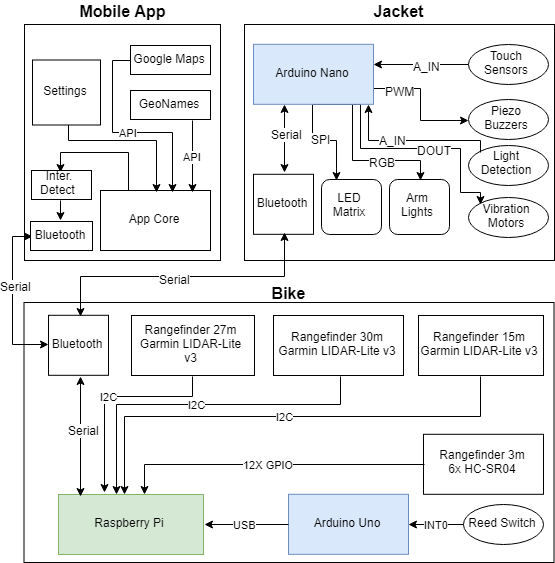
\includegraphics[width=5in]{blockdiagram}
    \caption{Block Diagram Showing the Architecture of CycleSafe}
    \label{fig:block_diagram}
\end{figure*}
\section{Architecture}
CycleSafe will consist of 3 main components,
\begin{enumerate}
    \item Mobile app that collects bike and location data
    \item Main system mounted on bike that uses distance sensors and phone data to determine safety
    \item Jacket wearable with warning feedback and traffic lights
\end{enumerate}
The block diagram can be found in \ref{fig:block_diagram}. In this section, we will describe what smaller devices exist on each level, and how each architectural component connects with one another.

\subsection{Mobile App}
The mobile app is an Android application that is responsible for giving the Raspberry Pi map and location data, as well as providing a user interface for the user to access many features of CycleSafe. The mobile app communicates with the Raspberry Pi via Bluetooth. In order for the app to give commands to the jacket, the app will have to issue a special command to the Raspberry Pi that then forwards the command to the jacket.

\subsection{Raspberry Pi}
The bicycle will have a mounted Raspberry Pi 3 (Pi) which will be the main processing hub and run the notification and alert system. The devices connected to the Pi are as follows:
\begin{itemize}
    \item 3x \lidar{} (via I2C)
    \item 6x Ultrasonic Sensor \sonar{} (via GPIO)
    \item Speedometer (via USB)
    \item Android Phone (via Bluetooth)
    \item Arduino Nano (via Bluetooth)
\end{itemize}

\subsection{Arduino Nano}
The Arduino Nano is the microcontroller that controls all features of the jacket, which has the following components:
\begin{itemize}
    \item 16x16 LED Matrix (output via SPI)
    \item 2x Arm LED strip warning lights (transistor control)
    \item 2x Piezo Buzzer (analog output)
    \item 4x Cell Phone Vibration Motors (transistor control with PWM power)
    \item 2x Turn signal input from the gloves (digital input)
\end{itemize}
The Arduino has Bluetooth connection with the Raspberry Pi, where it will receive commands to give user warning feedback.

\section{Design Trade Studies}

\subsection{Vehicle Detection}
The predominant monetary cost of the CycleSafe system arises from the required rangefinders. Because of the difference in speed of motor vehicles and cyclists, sensors typical for cars cannot be used for cyclists since typical lane change sensors only check the car's blind spot, which is very close to the car, and not the region visible in the car's side mirrors. Additionally, the cost of a car makes the cost of a its safety system insignificant, but this is not the case for a bicycle since bicycles are significantly cheaper than cars. The weight requirement for a safety system is similarly far more constrained on a bicycle than on a car.

A computer-vision based vehicle and obstacle detection system was considered as a potential solution. However, we noted that the power and processing requirements of such a system and the real-time nature of the safety system would make such a computer-vision based vehicle detection system impractical. Furthermore, CycleSafe requires more than to determine the location of nearby vehicles, but also to determine their speed, direction of motion, and acceleration, all of which would require processing of multiple frames at a time, increasing the processing requirements significantly. Nonetheless, a computer-vision based system would be superior in one particular situation: when detecting if vehicles are exiting side streets into the cyclist's path. This scenario is essentially impossible to address without a large number of sensors or wide-angle sensors with good resolution. However, we decided that it was worth sacrificing this scenario due to the impracticality of using such sensors or computer vision, and instead address it through signalling.

Based on these concerns, we determined that the CycleSafe system would utilize multiple single-point rangefinders that would require much less processing power to deal with. As further considerations, the CycleSafe system has to utilize longer-range sensors than in cars, and have a cost at most on the order of the cost of a bicycle. The large speed differentials between bicycles and vehicles also require higher data rates on sensors. Fortunately, there is a medium-range rangefinder commercially available. The \lidar{} has a \SI{40}{\meter} range and a measurement rate of \SI{500}{\Hz}, while weighing only \SI{38}{\gram}. It is designed for use in drones and similar real-time applications, making it well suited to CycleSafe. However, it costs \$130, which limits the quantity of these sensors the system will reasonably utilize. In designing the system, we took into account that only two or three of these sensors could be used in the entire system and that we would have to put them in strategic locations.

\label{sonar_tradeoff}
As a result, the shorter range sensors do not use the \lidar{}, but instead use the \sonar{}, a short range ultrasound rangefinder, with an effective range up to \SI{4}{\meter}. These sensors cost less than \$4, so despite their slow response time, which can be as low as \SI{20}{\Hz} and poor resolution, the CycleSafe system can utilize multiple such sensors to make up for the slow response time. In our system, we utilize 6 such sensors in order to run the proximity detection and signalling system, which only requires a range of \SI{3}{\meter}, and alternately take measurements from each sensor in order to achieve the desired update time.

\subsection{Component Locations}

Since the CycleSafe system involves a cyclist, a bicycle and a mobile app connection, there were many decisions to make with regard to the positioning of the various components.

The rangefinder sensors could have been located on either the cyclist and the bicycle, or both. However, we decided that the potential benefits of having the sensors at a higher vantage point were outweighed by the relatively static bicycle frame as a mount, since a cyclist does not remain still when cycling.

The measurement of the cyclist's speed could have been done using either a physical measurement on the bicycle wheel or using GPS. However, due to the latency of GPS and mobile transmissions in our experience and the necessity of real-time data, it was determined that the speedometer should be physical rather than a GPS measurement.

The use of the jacket as a signalling platform rather than the bicycle was made considering the surface area and height. Since signal clarity is one of the system's primary objectives, the greater surface area of the cyclist especially when viewed from the back makes directional signals significantly clearer, as compared to the very thin profile of the bicycle viewed from behind. The added complication of needing to connect the sensor system and the signalling system wirelessly was determined to be fairly insignificant since wired communication would still be needed even if the signalling system was on the bicycle. Since the communication requirement between the sensing and the feedback system uses very little bandwidth, using Bluetooth (used in communication systems) would not increase latency significantly.

Consideration was also made as to whether the feedback system should originate from a mobile device rather than the jacket. However, we concluded that since mobile devices are actually a common cause of bicycling accidents by diverting the cyclist's attention, it would be more effective to use a platform meant solely for the safety system will less potential to distract the cyclist.

\subsection{Battery Life}

Finally, in order to power all the components of CycleSafe, we needed a battery. Unfortunately, batteries can be expensive in many ways, but tend to rise in price with
\begin{itemize}
    \item Smaller size
    \item Less weight
    \item Longer battery life
\end{itemize}
For CycleSafe, since we want to be the least intrusive as possible to the original bike weight, we do not want to make the system too heavy; same goes for the jacket. Fortunately, the bike mounted system is very light, so most batteries are sufficient for the bike. In particular, most commuter bicycles are around \SI{30}{\lb} \cite{bicycle_weight}, and we aimed to keep our system below 10\% of the bicycle weight. Our entire bike mounted system without the battery is less than \SI{1}{\lb}, so \SI{2}{\lb} of battery weight gives us plenty of options.

As for the jacket, since the cyclist is wearing it, the weight has to be significantly less. We estimated that if the average commuter cyclist is \SI{140}{\lb}, we wanted the jacket to be less than 5\% of the cyclists' weight, or \SI{7}{\lb}. Since the jacket and components weighs about \SI{5.5}{\lb}, we are limited to about \SI{1.5}{\lb} for the jacket battery.

In addition to the weight tradeoffs, we also wanted our battery life to be long enough so that the cyclist did not have to charge the CycleSafe system too often. We deemed based on current products on the market \cite{bicycle_lights_cygolite, bicycle_lights_niterider} that 1 week was a reasonable amount of time to have to charge the devices.

\section{System Description}
\subsection{Android Phone}
The features of CycleSafe that are controlled through the mobile app include
\begin{itemize}
    \item \textit{Live navigation on the road}: the app uses the Google Maps API to provide directions to the biker 
    \item \textit{Custom jacket lights}: If the user wishes to use a different style of turn signals or brake lights, they can customize it through the app
    \item \textit{Custom jacket notifications}: The user can choose how they want to be notified in the event of a danger. This includes a combination of sound, light, and vibration feedback. The user can in addition choose to customize the type of vibration they feel.
\end{itemize}
In addition, the phone will provide information about when the biker is approaching an intersection. This is crucial, since the warning system behaves differently when the user is approaching an intersection. The phone sends intersection to the Raspberry Pi via Bluetooth.


\subsection{Raspberry Pi 3}
The Pi will be running data collection and data processing, sending commands to the Arduino Nano on the jacket. The algorithm will repeatedly run the following:
\begin{enumerate}
    \item Send trigger signals out to two of the HC-SR04. GPIO interrupts will handle the values returned.
    \item Request distance readings from all three LIDARs via I2C. Request the longer required range sensors first.
    \item Check velocity via serial.
    \item Check Bluetooth for incoming side-street data from Android.
    \item Check Bluetooth for user-activated signals from Arduino Nano.
    \item Check I2C for received LIDAR range values.
    \item Determine warnings to emit.
    \item Send warnings to Arduino Nano via Bluetooth.
\end{enumerate}

The primary reason the ordering is as such is to reduce the amount of time the Pi spends waiting. The ultrasonic sensors are the slowest sensors to respond to a measurement request, followed by the LIDAR. The Android App and the Arduino Nano do not require time to take measurements since the data received from them is not as time-sensitive and hence they can simply supply a recently-computed value.

\subsubsection{HC-SR04}

The HC-SR04 require a trigger signal to be sent, and respond with data encoding using the length of a pulse. As such, the Pi is required to monitor the HC-SR04 echo pin when it expects a measurement to arrive. Signal-edge triggered interrupts will allow the Pi to obtain a timestamp when the pulse begins and a timestamp when the pulse ends, while still performing other useful work.

The processing (subtracting the time and scaling) can then be done during the warning decision stage. This keeps the interrupts short and ensures they do not interfere with each others' timing. This is also the reason for only querying two of the HC-SR04 in one cycle of the algorithm, since having all six HC-SR04 using two interrupts each could potentially interfere with their timing data.

\subsubsection{\lidar{}}

The \lidar{} communicates with the Pi via I2C. All three rangefinders can use the same SDA/SCL lines, since they can be configured to use different I2C addresses. As it takes some time for the LIDAR to make a measurement, the Pi initiates the measurement at the beginning of the processing loop, and retrieves the measurement only right before it begins computation.

\subsubsection{Warning decision algorithm}
The algorithm used by the Pi to determine what kind of warning to emit to the cyclist is described here. The severe warning is given either when the cyclist is about to collide, or something is about to collide with the cyclist. As such, severe warning will be given under the following conditions:

\begin{enumerate}
    \item The frontal sensor detects an object at a distance covered within \SI{3}{\s} at the cyclist's current speed. This warning tells the cyclist to stop.
    \item The medium-range (\SI{15}{\meter}) blind-spot sensor detects a vehicle that is not decelerating and will collide with the cyclist within \SI{1}{\s}. The warning tells the cyclist to hold their lane.
\end{enumerate}

The severe warnings are meant to be followed without the cyclist needing to consider other inputs. As such, they need to be extremely trustworthy when they are activated. In addition to false negatives, False positives must also be kept to a minimum.

The notifications are given to the cyclist under the following conditions:

\begin{enumerate}
    \item Blind spot warning: when long range LIDAR detects a vehicle approaching, reaching the cyclist in in \SI{2}{\s} or less.
    \item When an intersection is approaching.
    \item When vehicles are in close proximity and may make a right turn.
\end{enumerate}

\subsection{Rangefinders}
\begin{figure*}
    \centering
    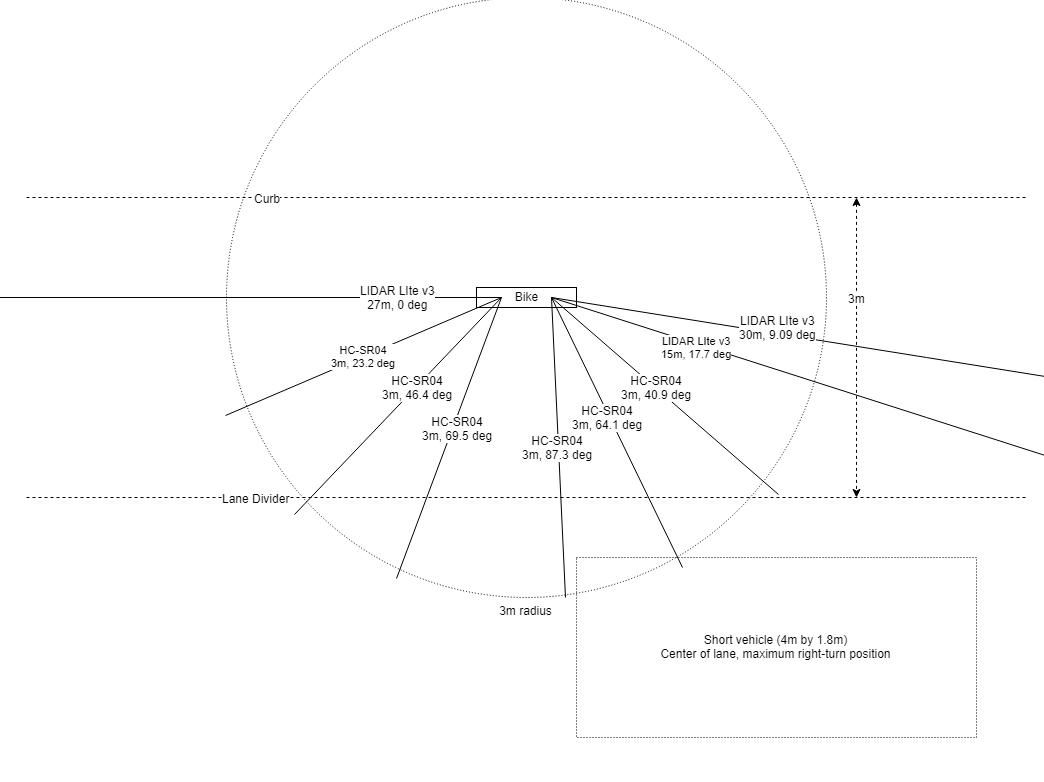
\includegraphics[width=\textwidth]{bike_config}
    \caption{Rangefinder Configuration with Bicycle Showing Ranges Covered}
    \label{fig:bike_config}
\end{figure*}
\subsubsection{Frontal sensor}
From Section \ref{specs:warning_thresholds}, we determined that the frontal sensor range requirement is at least \SI{19}{\meter}. The sensor used is a \lidar{}, which has a maximum effective range of \SI{40}{\meter}. This will be placed on a frontal mounting point on the bicycle pointing directly forward, providing unobstructed line-of-sight in front of the bicycle. It is connected directly to the Pi 3 via the 5V line and I2C bus, which will run along the length of the bicycle.

\subsubsection{Blind spot warning during lane change}
From Section \ref{specs:warning_thresholds}, we determined that the effective range of the blind spot sensor must be at least \SI{30}{\meter}. However, the blind spot sensor must face slightly diagonally in order to detect vehicles in an adjacent lane.

Given the lane width of $\slane$ = \SI{3}{\meter} and the sensor range of $s_{\text{bs\_max}}$ = \SI{30}{\meter}, we can determine the angle at which the sensor must be offset to detect a vehicle in the adjacent lane. Assuming the displacement from the cyclist to the closest point on the vehicle in the direction perpendicular to the lane direction is about one lane width, and the width of the vehicle $w_v$ is about \SI{1.8}{\meter}, we find the offset of the sensor, $\theta_{bs}$ from the axis of the direction of travel:
\begin{align}
\theta_\text{bs} = \arctan{\frac{\slane + w_\text{v}}{s_\text{bs\_max}}} = \arctan{\frac{4.8}{30}} = \ang{9.09}
\end{align}

Additionally we want to provide a severe warning to cyclists if it is likely that a vehicle will collide or be forced to swerve if the cyclist performs a lane change immediately. With the \SI{30}{\meter} blind spot sensor, it is well within reason to expect cars to slow down between the time they are detected \SI{30}{\meter} away and when they overtake the cyclist. As such, the feedback given to the cyclist when the vehicle is \SI{2}{\s} away will only be a notification. However, in some cases the vehicle will not slow down, and possibly not notice the cyclist.

To address this, a second sensor is utilized to provide a severe warning to the cyclist when the vehicle is \SI{1}{\s} away. Based on the earlier assumption that an oncoming vehicle will approach at at most \SI{15}{\meter/\s}, the sensor is required to have an effective range of $s_\text{bs\_near} = \SI{15}{\meter}$. Using the same method:

\begin{align}
\theta_\text{bs\_near} = \arctan{\frac{\slane + w_v}{s_{\text{bs\_near}}}} = \arctan{\frac{4.8}{15}} = \ang{17.74}
\end{align}

\subsubsection{Right turn cut off warning}
When a vehicle is about to make a right turn into a side street in front of a cyclist, there is a large range of possible positions the vehicle may take in relation to the cyclist. However, the vehicle will always have to come into fairly close proximity to the cyclist (less than one lane width). The CycleSafe system attempts to detect this by using an array of short range sensors. These short range sensors are positioned such that any one of them will detect a compact car within one lane width to the back-left, left and front-left of the cyclist (see Figure \ref{fig:bike_config}). The coverage should start just outside the detection area of the \SI{15}{\meter} blind spot sensor, and extend all the way to the detection area of the frontal sensor. Generally, compact cars are at least $l_{car} = \SI{4}{\meter}$ in length. At a distance of $\slane = \SI{3}{\meter}$, the angle $d\theta_{close}$ subtended by such a car is:

\begin{align}
\dd{\theta_\text{close}} = 2\arctan{\frac{l_\text{car}}{2\slane}} = 2\arctan{\frac{4}{6}} = \ang{67.38}
\end{align}

Hence, to ensure that any cars passing within the minimum distance of \SI{3}{\meter} is detected, we require a total of:
\begin{align}
    \left\lceil \frac{ \ang{180} - \ang{17.74} }{ \ang{67.38} } \right\rceil - 1 = 2
\end{align}
close proximity sensors.

However, as stated in Section \ref{sonar_tradeoff} we are using three sets of sensors, enabling staggered measurements in order to offset the slow measurement response time. This results in a total of six sensors in three sets of two each, and facing angles approximately $\ang{23}$ apart.

\subsubsection{Overall configuration}
The overall configuration of the sensors is shown in the diagram below (Figure \ref{fig:bike_config}). The frontal collision sensors and blind spot sensors are the \lidar{}. The six proximity sensors are the \sonar{} Ultrasonic Rangefinder.

\subsubsection{Other considerations}
It is worth noting that many laser-based range sensors typically perform more poorly in high sunlight conditions. However, this is partially compensated by the improvement in visibility and general reduction of braking distance in pleasant weather conditions.

\subsection{Arduino Nano}
The Arduino Nano is the microcontroller that is responsible for controlling all the peripherals on the jacket. More details about each individual component can be found in the following sections. Since the jacket does not send any data to the Raspberry Pi, it is a passive component in the architecture, and thus the Nano only receives commands via Bluetooth from the Raspberry Pi. 

\subsection{LED Matrix}
The LED Matrix serves as the main light signalling component of the jacket wearable. Similar to how cars have turn signals and brake lights, the LED Matrix in the back can serve any of these light functions. Because the matrix is configurable to its $16 \times 16$ granularity and full RGB, it can emulate almost any signal. 

For our project, the LED Matrix has the following lighting modes,
\begin{itemize}
    \item Ambient lights: Matrix is a dim red. Especially important during nighttime, to give other vehicles on the road awareness of the rider.
    \item Brake lights: Matrix is a brighter red than the ambient light. This mode is triggered if the speed of the rider is slowing down. 
    \item Turn Signals: Flashing arrows that indicate which direction the biker is trying to turn into
\end{itemize}

In order to display images on the LED Matrix, 2D data has to first encoded into 1D linear data, and then sent to the Arduino. because the Arduino has limited memory, we unfortunately cannot store all the shapes we need, because it is too expensive.

\subsection{Piezo Buzzers and Vibration Motors}
One of the goals of this project is to give the rider as much awareness about the road as possible, while also allowing the rider to focus on the road by keeping CycleSafe minimally intrusive. The Piezo Buzzers and Vibration Motors are forms of non-visual feedback to the rider, namely auditory and sensory, that use beeping sounds and vibrations to give the rider warning about dangerous situations.

This is akin to how many blind spot features in cars nowadays beep when a driver is about to turn into a lane that is not empty. This type of feedback is very important, because people can forget to check that a lane is empty before changing. In addition, for a biker, who doesn't have rear or side mirrors, they have to expend a larger motion just to check if a lane is clear. Therefore, these two forms of feedback minimize the need for the rider to check for visual warnings, and also serves as a fallback warning system in case the rider just forgets to check in the first place.

\subsection{Speedometer}
The function of the speedometer is to determine the speed of the bicycle. It consists of a single reed switch, placed on the bicycle's front fork, activated by a magnet, and connected to the interrupt pin on Arduino B. The circuit is shown in Figure \ref{fig_speedometer}.

\begin{figure}[!t]
\centering
    \def\cktWidth{4}
    \def\rHeight{4}
    \def\rWidth{2.5}
    \def\rA{3.5}
    \def\rB{2}
    \def\rC{0.5}
    \begin{circuitikz}
        % \tikzmath{\r_height = 4; \r_width=3;}
        \draw (0,0) rectangle (\rWidth,\rHeight) node[yshift=-12pt, pos=0.5, label={[align=center]Arduino B\\(Arduino Uno)}] {};
        
        \node (5V) at  (\rWidth + 1, \rA) {\SI{5}{\volt}};
        \node (GND) at (\rWidth + 1, \rB) {GND};
        \node (D2) at  (\rWidth + 1, \rC) {D2/INT0};

        \draw (\rWidth, \rA) 
            to[short] (5V.west)
            to[open]  (5V.east)
            to[ospst]  (\rWidth + \cktWidth, \rA)
            to[short] (\rWidth + \cktWidth, \rC)
        ;
        
        \draw (\rWidth, \rB) 
            to[short] (GND.west)
            to[open]  (GND.east)
            to[R=$\SI{10}{\kilo\ohm}$]  (\rWidth + \cktWidth, \rB)
        ;
        
        \draw (\rWidth, \rC) 
            to[short] (D2.west)
            to[open]  (D2.east)
            to[short]  (\rWidth + \cktWidth, \rC)
        ;
    \end{circuitikz}
\caption{Speedometer circuit configuration.}
\label{fig_speedometer}
\label{fig_speedometer_1}
\end{figure}

The speedometer will require the user to configure the wheel diameter or the wheel circumference using the app interface. The bicycle velocity, $v_b$ will then be computed by Arduino B, as follows:

\begin{align}
    v_b = \frac{4\pi d}{t - t_{4}}
\end{align}

where $t$ is the current timestamp, $t_{4}$ is the timestamp four interrupts prior, and $d$ is the diameter of the wheel. Wheel diameters typically range from \SI{507}{\milli\m} to \SI{622}{\milli\m}, with \SI{622}{\milli\m} being the most common. %TODO citation

Waiting for four interrupts computes the average speed over the last four wheel rotations instead of merely the last rotation. This reduces speed fluctuations, which would adversely affect the accuracy of the warning algorithm. It also reduces the error in case an interrupt is missed or an additional interrupt somehow occurs. in this case, the average of four limits the error to 25\% of the actual value. An average of four was used because four rotations of a \SI{622}{\milli\meter} wheel on a bicycle covers a distance of \SI{7.816}{\m}, which is approximately one second at typical bicycle speeds of \SI{5}{\meter/\s} to \SI{9}{\meter/\s}. However, the trade-off is that the it may take up to a second for the speedometer to respond to changes in velocity. Large changes in speed are only likely when the bicycle is coming to a sudden stop, and therefore a slower response to a sudden decrease in speed will favor false positives over false negatives, which is preferable.

\section{Project Management}
\subsection{Schedule}
We are using TeamGantt to organize our tasks and keep track of our progress. We have attached our Gantt Chart schedule at the end of the paper. 

We are mostly on track with our project. We are anticipating some latency in integrating all aspects of the project together---once we physically construct our bicycle add-on and jacket. Fortunately, we have latency built in, so we should be able to overcome any difficulties we have in assembling our project. We plan to test in April, and give us 

A link to the chart can be found \href{https://prod.teamgantt.com/gantt/schedule/?ids=1489092&public_keys=7aQHatcI23su&zoom=d100&font_size=12&estimated_hours=0&assigned_resources=0&percent_complete=0&documents=0&comments=0&col_width=355&hide_header_tabs=0&menu_view=1&resource_filter=1&name_in_bar=0&name_next_to_bar=0&resource_names=1#user=&company=&custom=&date_filter=&hide_completed=false&color_filter=}{\underline{here}}.

\subsection{Team Member Responsibilities}
% not sure how we want to structure this, could just do 3 sections
\textbf{Ben}
\begin{itemize}
    \item Raspberry Pi control software
    \item Bike distance sensor setup
    \item Bike speedometer
    \item Formal Specifications
\end{itemize}

\textbf{Siddhanth}
\begin{itemize}
    \item Develop the mobile app, including Bluetooth communication, map API development, UI
    \item Write intersection detection algorithms
    \item Collect bike speed, location, map data to send as inputs to the safety logic in the Raspberry Pi
\end{itemize}

\textbf{Michael}
\begin{itemize}
    \item Design haptic feedback on the jacket
    \item Integrate jacket peripherals with the Arduino Nano controller
    \item Design and create jacket lights to satisfy official vehicle
requirements     \item Build communication between the jacket and the Raspberry Pi controller
\end{itemize}

\subsection{Budget}
\begin{table}[H]
    \centering
    \begin{tabularx}{0.4\textwidth}{ll}
        \toprule
         \textbf{Item}  & \textbf{Price}  \\
         \midrule
         % Bike
         Garmin LIDAR-Lite v3-HP (1)    & \$149.99 each\\
         Garmin LIDAR-Lite v3 (2)       & \$129.99 each\\
         HC-SR04 Ultrasonic Sensor (6)  & \$6.99 each\\
         EK1621x2 Reed Switch           & \$0.50\\
         
         % Jacket
         Rainproof Jacket               & \$29.99\\
         WS2812B LED Strip              & \$28.95 each\\
         Piezo Buzzer PS1240 (2)        & \$1.50\\
         Cellphone Vibration Motor (4)  & \$1.95\\
         
         % control
         Raspberry Pi Model 3           & \$29.99\\
         Arduino Nano                   & \$4.95\\
         
         % Power
         16750mAh Portable Charger      & \$34.99\\
         \midrule
         \textbf{Total} & \textbf{\$576.88}\\
         \toprule
    \end{tabularx}
    \caption{Prices for materials}
    \label{tab:prices}
\end{table}

\subsection{Risk Management}
Having parts come in late was expected, but we fortunately had many of the major parts already in hand, we could develop without some of the parts coming in. For example, we already had a Raspberry Pi, Arduino Nano, and a mobile phone at the start of the project, so we could develop on those devices while waiting for our other parts to come in. 

One of the major concerns we had for our entire system was power, since we eventually wanted to have a portable power source and we had some potentially power-consuming devices, including LED strips and LIDAR sensors. To reduce risk, we did two things
\begin{enumerate}
    \item Reduce the power consumption of these devices. For the LED strips, we made sure to only activate a subset of the 256 available lights. For the LIDAR, we only requested for distance data when we needed it.
    \item Put more batteries on the bike, and plug in the jacket into the bike as a backup option for power.
\end{enumerate}

%% TODO CITE SOURCES
\section{Related Work}
There are not many projects that take a serious attempt to build a full-scale bicycle safety system. Some related work include a bicycle blind spot detection system \cite{bicycle_blind_spot}, which consisted of an ultrasonic sensor on the back of the helmet and LED notification about nearby cars. Another project called Sixth Sense \cite{bicycle_sixth_sense} is a wireless distance sensor that vibrates a smart device when objects, such as cars, are nearby. These projects only have very limited functionality with car detection, especially when cars are approaching at faster speeds, since the range of their distance sensors is small, and it does not seem like they have acceleration detection.

Most of the safety features of CycleSafe were inspired by current car safety features. For example Honda Sending \cite{honda_safety} now includes the following safety features
\begin{itemize}
    \item Collision Mitigation Braking System
    \item Road Departure Mitigation
    \item Blind Spot Information System
\end{itemize}
CycleSafe focuses on implementing collision avoidance and blind spot information.

\section{Summary}
CycleSafe provides a comprehensive safety system that makes biking safer than current biking practices. By giving the rider warnings well ahead of collisions with cars and objects, CycleSafe can prevent many of the accidents that lead to many cyclist deaths every year.

\subsection{Future Work}
Since cars have safety features, and now CycleSafe introduces safety to cyclists, a natural extension of the project is to bring safety features to motorcyclists. For a higher speed vehicle like a motorcycle, we expect to need sensors that have further ranges so we can detect oncoming traffic and objects from longer distances.

\subsection{Lessons Learned}
The biggest problem we have encountered so far is that the parts we order do not come in on time, even if they are Amazon Prime. So there should be a good amount of planning ahead to make sure that parts coming does not affect the progress of the project.

% use section* for acknowledgment
\section*{Acknowledgment}
The CycleSafe team would like to thank the Electrical and Computer Engineering department of Carnegie Mellon University for their financial support in making this project possible. In addition, we would like to thank Professor Ken Mai for his advising throughout the project
and Zilei Gu for her constant support and check-ins with our project.


% trigger a \newpage just before the given reference
% number - used to balance the columns on the last page
% adjust value as needed - may need to be readjusted if
% the document is modified later
%\IEEEtriggeratref{8}
% The "triggered" command can be changed if desired:
%\IEEEtriggercmd{\enlargethispage{-5in}}

%% BIBLIOGRAPHY
\bibliographystyle{IEEEtran}
\bibliography{biblio}

\clearpage
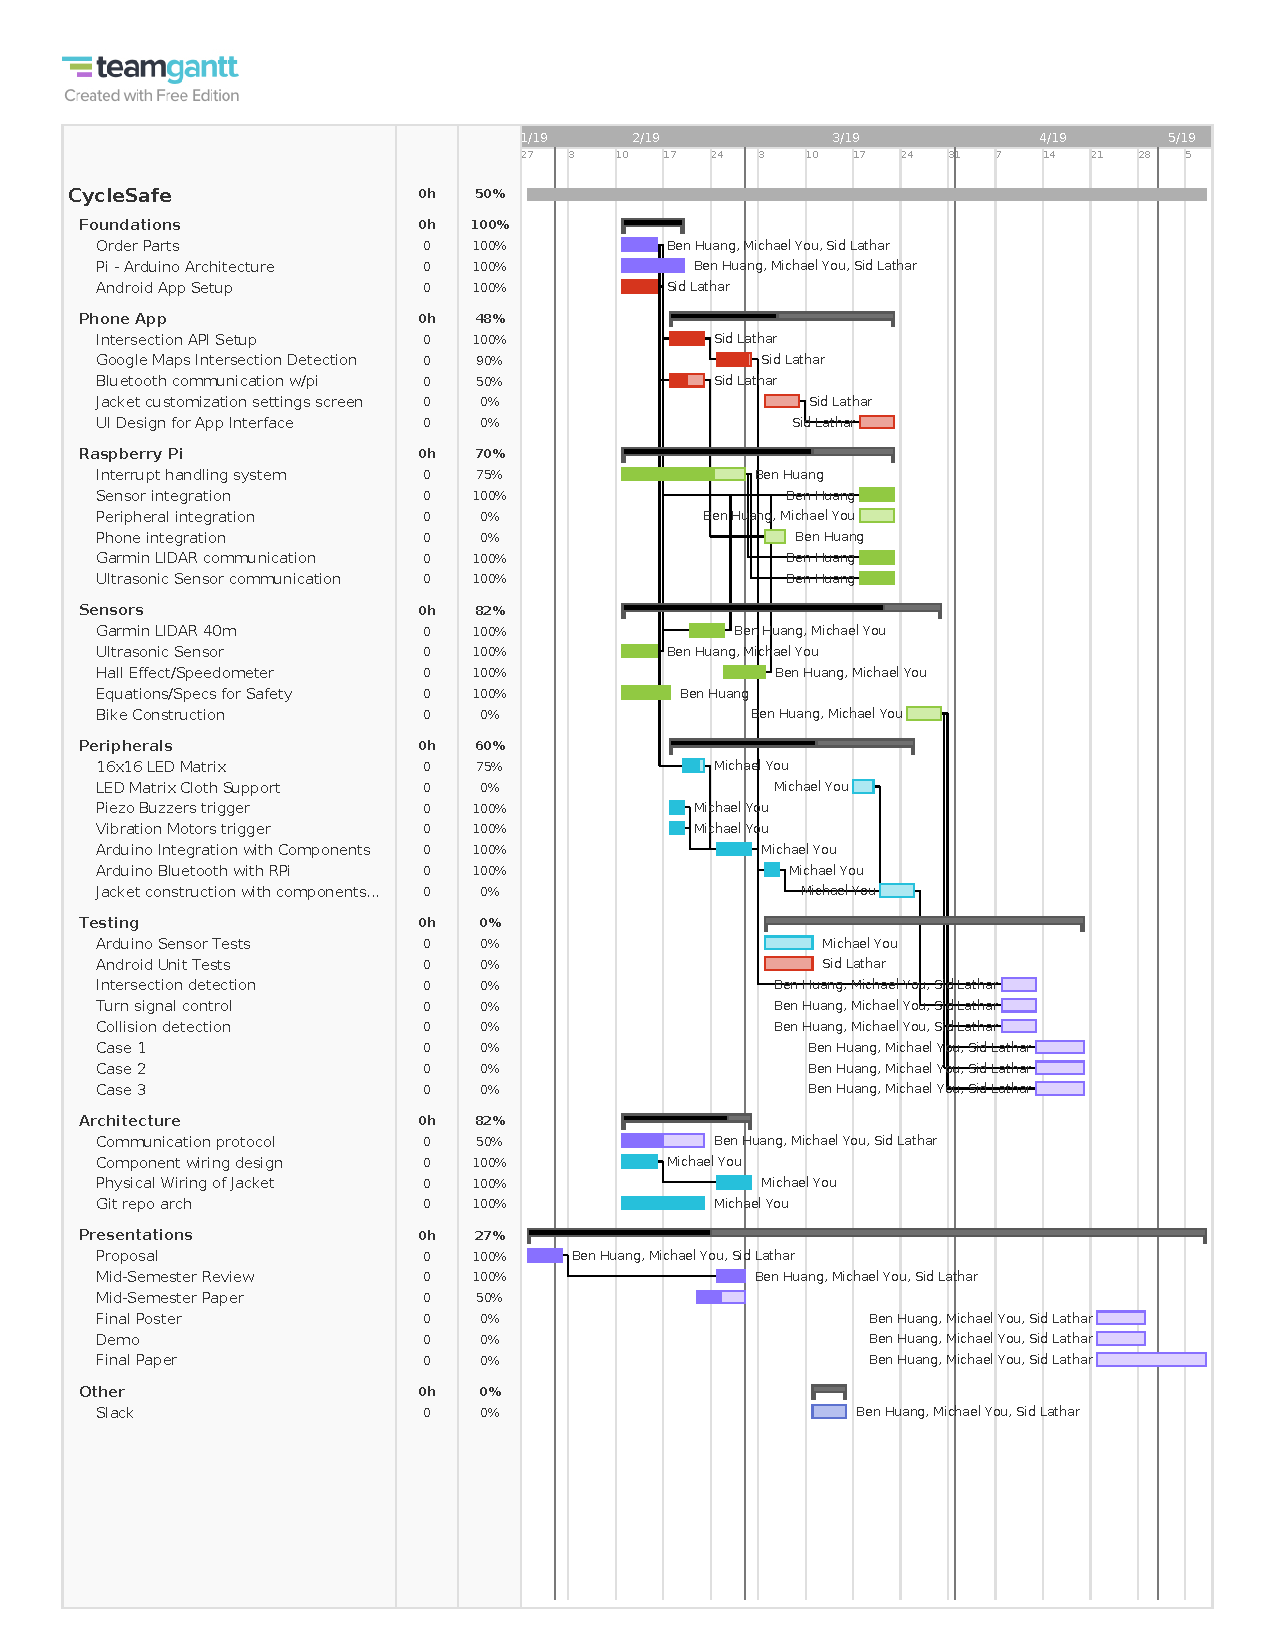
\includepdf[pages=-]{gantt.pdf}

%% APPENDIX
% if have a single appendix:
%\appendix[Proof of the Zonklar Equations]
% or
%\appendix  % for no appendix heading
% do not use \section anymore after \appendix, only \section*
% is possibly needed

% use appendices with more than one appendix
% then use \section to start each appendix
% you must declare a \section before using any
% \subsection or using \label (\appendices by itself
% starts a section numbered zero.)
%

%\appendices
%\section{Proof of the First Zonklar Equation}
%Appendix one text goes here.

% you can choose not to have a title for an appendix
% if you want by leaving the argument blank
%\section{}
%Appendix two text goes here.

\end{document}


